\documentclass{ctexart}
\CTEXsetup[format={\Large\bfseries}]{section}
\usepackage{graphicx}
\bibliographystyle{plain}
\begin{document}
\title{Telekine: Secure Computing with Cloud GPUs}
\author{梁允楷, 18342055}
\date{}
\maketitle    
\section{研究背景}

随着技术的完善和机器学习的兴起,GPU 现在已经普遍用于云上来加速计算。
目前的云平台都只能在信任云服务商的基础上,提供相应的云计算服务。
这样的云计算服务存在相应的隐患:

\begin{itemize}
    \item 云服务商的系统存在系统漏洞,黑客可能会对这个系统攻击,导致用户数据的泄露。
    \item 云服务商的隐私保护可能不一定和云服务客户的隐私保护一致。
    \item 云服务商有自己的利益和关注点,一些服务商或者是管理者可能利用特权窃取数据。
\end{itemize}

这样的安全隐患,对于一些安全要求高的客户而言是不可接受的。
这样会导致一些客户有云计算服务的需求,但无法满足他们的安全需求。
因此,会劝退这这部分对安全敏感的用户使用云计算服务。
例如存在以下的场景:一些客户(企业、医生等)可能需要使用云进行机器学习的推断,提供的数据可能涉及客户服务对象的隐私(企业用户隐私、患者隐私等)。

因此,需要我们实现相应的技术,实现在不可信的云平台上仍可以进行安全计算,避免对云服务商信任的依赖。

目前,利用硬件可以实现受信任的执行环境,这个技术被成为可信执行环境 (TEE)\cite{jang2019heterogeneous}。
该技术的主要原理为设置隔离边界,确保白名单以外的软件无法跨越边界。
以此,达到云服务商无法查看环境内部发生的事情以及相应的通信,但该技术无法保证对侧信道攻击的防御。

\section{方法介绍}

\subsection{侧信道攻击例子}

使用可信执行环境 (TEE) 技术可以在不可信的云环境下的实现可信的 GPU 计算问题。但该技术仍有局限性:作者在论文\cite{246310}中论证了即使在 CPU 和 GPU 上使用固件或硬件支持的 TEE 技术,仍不能保证对缓存侧信道攻击的保护。

云服务商可以通过观察虚拟机的 CPU 和 GPU 的交互获得相应的时间信息信息。
获得的时间信息主要体现在:

\begin{itemize}
    \item GPU 计算中频繁发生 GPU 执行管理和数据回传管理,这些通信模式可能导致信息泄露造成定时信道攻击。
    \item 云服务商可以通过 DMA 中断获得 GPU 处理时间间接获知用户的信息。
\end{itemize}

作者提出了一个概念验证,利用 CPU 和 GPU 交互的时间信息训练构建一个图像分类的机器学习模型。
和随机分类的模型相比,即使没有获得原图像输入的情况下,
利用时间信息构建的分类模型效果也有显著的提高,模型分类的准确率平均上升 1.6 倍。
其分类的效果如图\ref{fig: side-chan attack}所示。

\begin{figure}
    \centering
    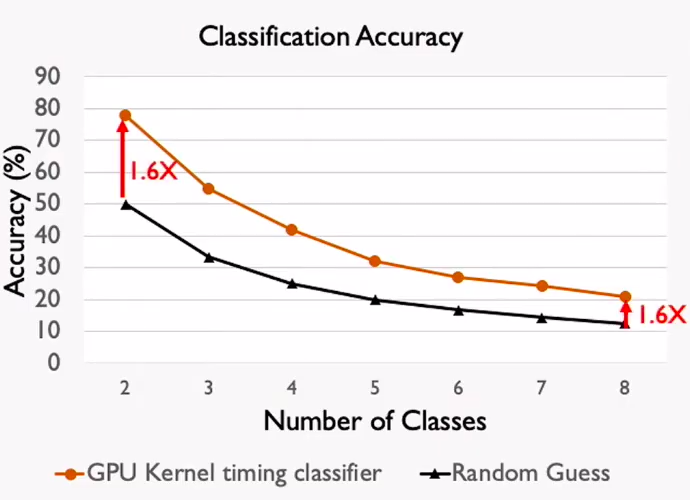
\includegraphics[width=8cm]{images/side-chan-attack.png}
    \caption{side-channel attack}
    \label{fig: side-chan attack}
\end{figure}

因此,TEE 技术不能解决定时信道攻击。需要创建新的模型,去除这些通过 GPU 的通信模式造成可以收集的时间信息。

\subsection{API 远程处理}

\begin{figure}
    \centering
    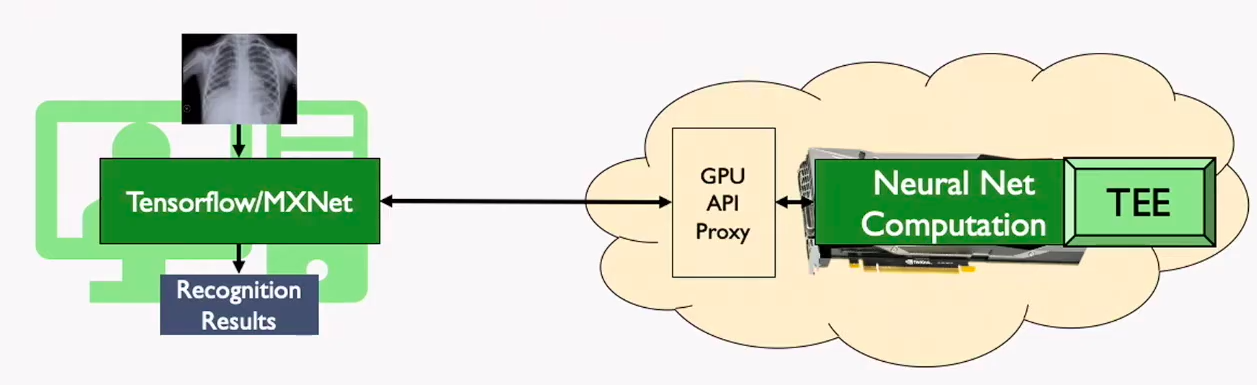
\includegraphics[width=8cm]{images/telekine-model.png}
    \caption{将执行的代码从云转移到客户机上执行}
    \label{fig: telekine-model}
\end{figure}

为了避免上述的攻击,作者提出了一个方法:将运行代码移到可信的机器(客户机器)。
确保了云服务商只接收数据进行计算,没有直接和源代码进行交互避免数据的泄露。

使用的技术为 API 远程处理(API-remoting),将自己的库替换为 GPU 对应的库文件,实现的效果为使用云端的 GPU,在本地主机虚拟出对应的 GPU。只需要将对应的计算通过 API 代理在云端进行处理,此时传送到云端的不是代码,只是一些计算请求。此时,计算系统的模型如图\ref{fig: telekine-model}所示。

\subsection{消除 GPU 执行的时间信息}

\begin{figure}
    \centering
    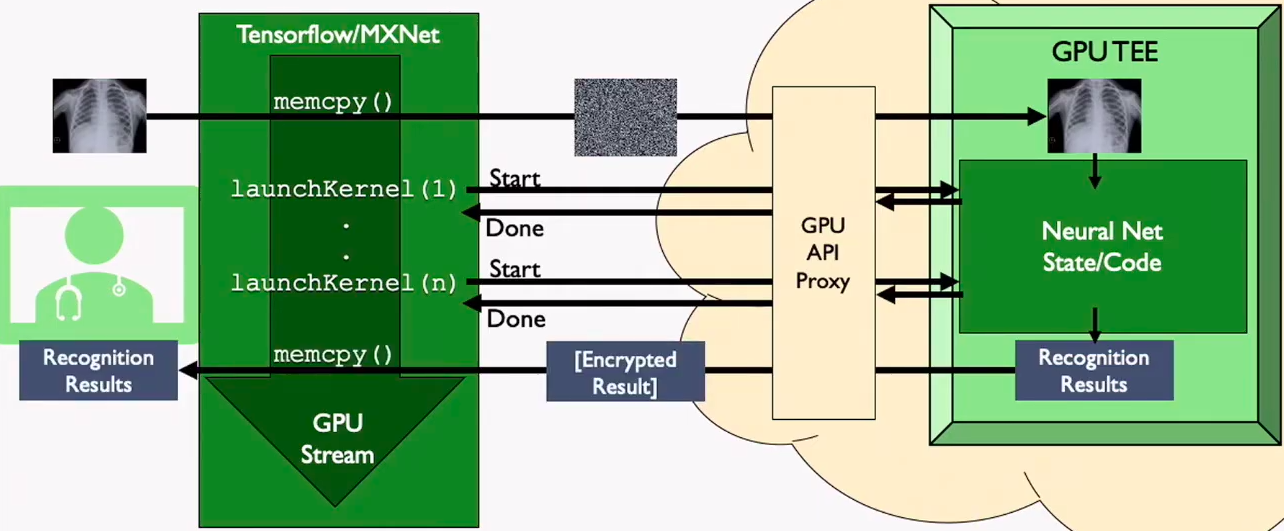
\includegraphics[width=8cm]{images/remote-api.png}
    \caption{通过监听客户机和 GPU 的交互获得时间信息}
    \label{fig: remote-api}
\end{figure}

上述的操作本质将不可信的 CPU 和 GPU 的交互转移到客户机(可信机器)和 GPU 的交互。云服务商仍可以监听 GPU 何时与客户机进行交互,获得 GPU 执行时间的信息,如图\ref{fig: remote-api}所示。因此,需要继续解决消除云服务商通过 GPU 的通信模式获取信息的可能性的挑战。解决上述挑战挑战,主要有以下的两个原因,解决这两个困难后即可消除 GPU 执行的时间信息:

\begin{itemize}
    \item 对于不同类型的 GPU 指令,有不同的大小或者不同的交互模式。因此,需要确保攻击者不能通过这些不同获得信息
    \item 通常的 GPU 指令流执行指令和数据传输指令之间存在依赖,因此可能泄露时间信息
\end{itemize}

为了解决消除云服务商通过 GPU 的通信模式获取信息的可能性的挑战挑战,对 GPU 需要满足以下条件:

\begin{itemize}
    \item 避免和其它用户一起共享并行使用 GPU,或者在释放 GPU 之前将计算状态清除,以免泄露计算的信息。
    \item 隐藏内核完成工作的信息,关闭 GPU 向不可信 CPU 发出的中断信号,改用恒定的速率传输数据,避免时间信息的泄露。
    \item 支持 no-op 的内核启动指令,使云平台始终看到内核在以固定的速率启动,避免通过内核的等待时间推断出相应的计算信息。
    \item 内核应及时消耗命令,防止因为等待其它内核导致加密信道内容满载造成时间信息的泄露。
\end{itemize}

GPU 满足上述条件后,作者提出数据遗忘流 (data oblivious streams) 方法消除通过通道获得的 GPU 时间安排信息。

\subsection{数据遗忘流}

作者构建的 Telekine 系统使用两个流传输信息:一个流用于启动应用内核和执行指令,被称为 ExecStream;另一个流用于和 GPU 进行数据的传入和传出,称为 XferStream。这两个流被特别地构造,防止传输数据的过程中泄漏模型执行的时间信息。这两个流的具体特点如下:

\begin{itemize}
    \item 这两个流经过系统进行分割和填充,使得系统传输的各个命令大小一致,再使用恒定的速度进行传输。这样操作后,DMA 获得的时间信息和系统推断的模型相互独立,无法通过 DMA 获得数据的时间推断模型执行的信息。
    \item 当一个内核与其他内核进行同步时,仍会继续执行指令,相应的指令为空指令,避免由于内核的唤醒,泄漏模型计算的时间信息。
    \item 由于数据传输带有方向,因此 XferStream 流需要维护两个方向。避免由于方向而泄露相关的计算信息。
    \item 这两个流相互独立地传输数据,并且 XferStream 特地构造为不和 ExecStream 同步,避免由于 XferStream 等待被 ExecStream 占据的 GPU 而泄露模型的执行时间。
\end{itemize}

\begin{figure}
    \centering
    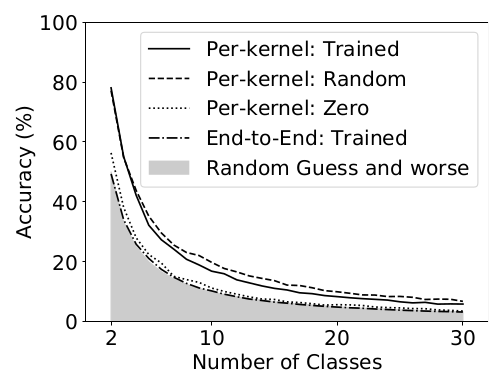
\includegraphics[width=8cm]{images/end-to-end-trained.png}
    \caption{End-to-End: Trained}
    \label{fig: end-to-end-trained}
\end{figure}

此时,不管是数据还是指令的传输,都与模型的执行无关。云服务商只能获得模型开始计算和模型结束计算的时间。从中获得的模型信息很少,整个计算环境是安全的。

作者同样利用开始时间和结束时间训练图像分类模型,具体达到的效果如图\ref{fig: end-to-end-trained}所示,其中 End-to-End: Trained 为端到端的训练模型,即使用开始和结束时间进行训练的模型,阴影部分为最差的模型(随机分类)。
达到的效果和随机分类的模型相差不大,

\subsection{系统执行流程和系统开销}

\begin{figure}
    \centering
    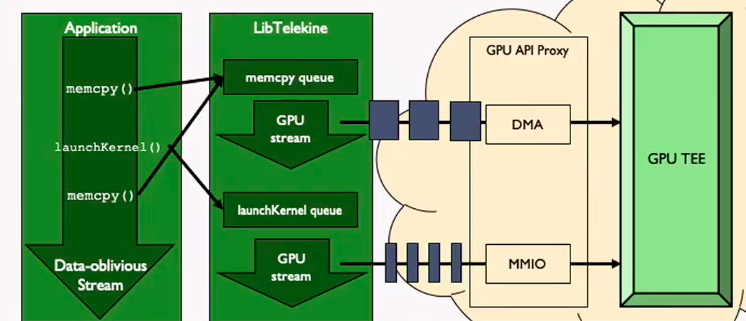
\includegraphics[width=8cm]{images/telekine-system-model.png}
    \caption{Telekine system model}
    \label{fig: system-model}
\end{figure}

整个系统的执行流程如图\ref{fig: system-model}所示,整个过程需要对传输数据和执行指令的各条语句分别进行封装。经过 Telekine 系统的裁减、填充,然后进行加密传输到云平台的 GPU 在进行解密,通过 API 接口远程处理调度对应云平台上的 GPU 进行可信的计算。

系统开销主要分成三个部分:调用远程 API 的开销、对数据进行加密、数据遗忘流调度的开销。

下图\ref{fig: overhead}是使用 Telekine 系统训练机器学习模型得到各个开销的组成部分。通过上图可以看出 Telekine 的开销主要来自于 API 远程处理和数据遗忘流的调度,加密和解密的开销较小。当 RTT = 10ms 时,Telekine 系统的总开销大约为原任务的 20\%,在安全计算的场景下是可以接受的。

\begin{figure}
    \centering
    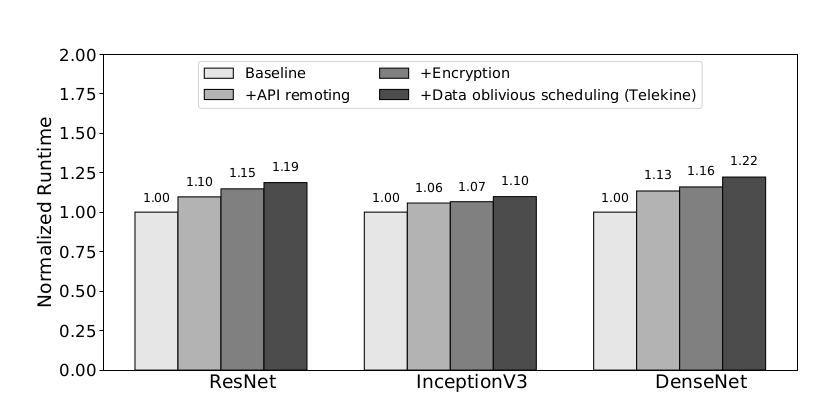
\includegraphics[width=8cm]{images/overhead.png}
    \caption{The overhead of Telekine}
    \label{fig: overhead}
\end{figure}

另外,Telekine 系统需要通过互联网传输指令和数据到云平台,故系统的开销对网络环境是十分敏感的。越大的往返延时 (RTT),会导致系统更大的系统开销。论文给出了不同 RTT 的情况下, 系统训练不同的机器学习模型对应的开销,具体数据在表格中展现。

\begin{table}
    \caption{不同的 RTT 下,系统训练不同机器学习模型的开销}
    \label{tbl: overhead with RTTs}
    \centering
    \begin{tabular}{r|rrr}
        \hline
        RTT(ms) & ResNet & InceptionV3 & DenseNet \\
        \hline
        10 & 1.19x & 1.10x & 1.22x \\
        20 & 1.29x & 1.13x & 1.37x \\
        30 & 1.44x & 1.16x & 1.49x \\
        40 & 1.53x & 1.18x & 1.66x \\
        50 & 1.62x & 1.30x & 2.09x \\
        \hline
    \end{tabular}
\end{table}

对应的,如果 GPU 计算的所需时间越长,Telekine 的开销占比越小。即,增加 batch size,可以减少 Telekine 开销的占比。在作者的论文中当 batch size = 64 时,在一些情况中 Telekine 的开销甚至可以忽略不计,具体的结果如图\ref{tbl: batch-size}和图\ref{fig: GPU-comp-time}所示。

\begin{figure}
    \centering
    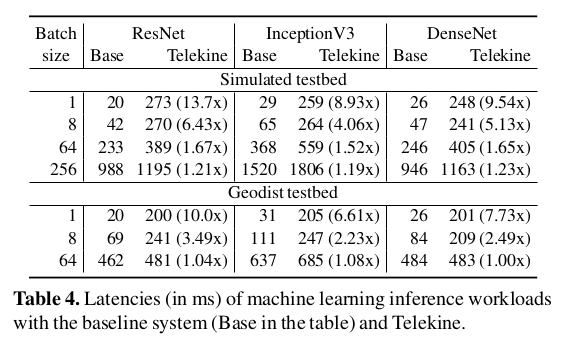
\includegraphics[width=6cm]{images/batch-size-overhead-tbl.png}
    \caption{不同的 batch size 对应的系统开销}
    \label{tbl: batch-size}
\end{figure}
\begin{figure}
    \centering
    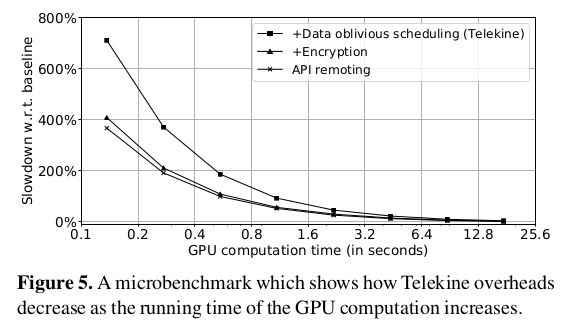
\includegraphics[width=6cm]{images/GPU-comp-time-plot.png}
    \caption{不同的 GPU 计算时间对应的系统开销}
    \label{fig: GPU-comp-time}
\end{figure}

\section{关于论文的一些讨论}

论文的主要优点如下:

\begin{itemize}
    \item 作者提出的系统很新颖,使用 API 远程处理技术,将执行代码从云端移到可信的本地主机,提供了一种新的思路处理安全的相关问题。
    \item 作者提出的系统,依靠 GPU TEE、API 远程处理和数据遗忘流调度等技术,实现了在不可信的云平台下进行可信计算的需求,扩大了云计算的使用范围。
    \item 系统模型开销相对较小,特别需要达到这种可信安全的计算环境中,这样的开销相对来说可以接受。
    \item 作者提出的模型系统,反映了云计算的本质是租借计算能力。在云平台中使用的是其计算能力,而无需使用其他的服务,因此可以实现在不可信的云平台下进行可信的计算。
\end{itemize}

论文的主要缺点如下:

\begin{itemize}
    \item 模型中侧信道攻击只是涉及了时间方面的考量,没有考虑到功率、温度等其它物理层面的侧信道的攻击方法。
    \item 论文中涉及的情况是用户自己提供机器学习模型,还有一些情况是云服务商提供模型,例如华为云的 model art,对于这些情况论文还可以进一步继续讨论。
    \item 作者提出的系统使用固定速率传输数据,以实现对数据的遗忘调度。因此,需要对传输速度进行限制。
    \item 由于数据不是直接存储在云平台上,若传输的数据量比较大,会造成传输数据的开销比较大。如果对数据反复进行重用且云平台不对相关的数据进行保存,可能导致数据在网路上反复进行传送。
    \item 为了维护数据流具有恒定的速率,需要向两个流中增加一些无用的操作,增加了额外的传输开销。
\end{itemize}

通过对论文的分析,我们可以利用论文的相关技术,对类似的问题进行处理:

\begin{itemize}
    \item 和时间同样的类比,我们可以在 GPU 上执行无用的指令,维持 GPU 的计算量在一个固定的值,来消除 GPU 执行指令所产生的功率和温度的信息,但也会因此增加进行云计算的预算开支。
    \item 对于一些不需要使用云数据库的应用,可以考虑将涉密的数据保存在本地的主机,以此避免在云平台上进行密文查找等相关操作。当然,这只能在数据量不大的情况下使用,大多数企业需要使用数据中心作为自己的数据库,因而可行性不大。
    \item 处理类似安全问题时,可以考虑引入多个可信的媒介,对涉密数据进行分布式的存储,将涉密数据的处理分布到对应的可信媒介中,实现“安全”的负载平衡。
\end{itemize}

\bibliography{reference}

\end{document}
